\hsectionENDE{Logical Modeling}{Logische Modellierung}%
%
%%
\begin{questionENDE}{Entity Types}{Entitätstypen}%
\qENDE{%
How will \emph{entity types} in the conceptual model be represented in a (relational) logical model?%
}{%
Wie werden \emph{Entitätstypen} aus dem konzeptuellen Modell im (relationalen) logischen Modell dargestellt?%
}%
\end{questionENDE}%
%%
\begin{questionENDE}{Attributes}{Attribute}%
\qENDE{%
How will \emph{simple single-valued attributes} in the conceptual model be represented in a (relational) logical model?%
}{%
Wie werden \emph{einfache einwertige Attribute} aus dem konzeptuellen Modell im (relationalen) logischen Modell dargestellt?%
}%
\end{questionENDE}%
%%
\begin{questionENDE}{Attributes}{Attribute}%
\qENDE{%
How will \emph{simple multi-valued attributes} in the conceptual model be represented in a (relational) logical model?%
}{%
Wie werden \emph{einfache mehrwertige Attribute} aus dem konzeptuellen Modell im (relationalen) logischen Modell dargestellt?%
}%
\end{questionENDE}%
%%
\begin{questionENDE}{Attributes}{Attribute}%
\qENDE{%
How will \emph{composite single-valued attributes} in the conceptual model be represented in a (relational) logical model?%
}{%
Wie werden \emph{zusammengesetzte einwertige Attribute} aus dem konzeptuellen Modell im (relationalen) logischen Modell dargestellt?%
}%
\end{questionENDE}%
%%
\begin{questionENDE}{Attributes}{Attribute}%
\qENDE{%
How will \emph{composite multi-valued attributes} in the conceptual model be represented in a (relational) logical model?%
}{%
Wie werden \emph{zusammengesetzte mehrwertige Attribute} aus dem konzeptuellen Modell im (relationalen) logischen Modell dargestellt?%
}%
\end{questionENDE}%
%%
\begin{questionENDE}{Modelling}{Modellierung}%
\qENDE{%
Assume that the relationship between listeners and songs follows the schema \crowsFoot{listener}{OM}{song}{OM}. %
Every listener has a name and age. %
Every song has a title, singer, and duration. %
Which tables, attributes, and constraints do you need to represent this situation correctly in the relational model?%
}{%
Nehmen Sie an, dass die Beziehung zwischen Zuhörern und Songs dem Schema \crowsFoot{Zuhörer}{OM}{Song}{OM} entspricht. %
Jede Zuhörer hat einen Namen und ein Alter. %
Jeder Song hat einen Titel, Sänger und eine Dauer. %
Welche Tabellen, Attribute und Einschränkungen brauchen Sie, um dieses Situation im relationalen Modell korrekt darzustellen?%
}%
\end{questionENDE}%
%
\begin{questionENDE}{Surrogate Keys}{Ersatzschlüssel}%
\qENDE{%
What is a \emph{surrogate key}? %
Why does it often make sense to use one?%
}{%
Was ist ein \emph{Ersatzschlüssel}? %
Warum ist es oft sinnvoll, einen zu verwenden?%
}%
\end{questionENDE}%
%
%
\begin{questionENDE}{Conceptual to Logical}{Konzeptuell zu Logisch}%
\begin{center}%
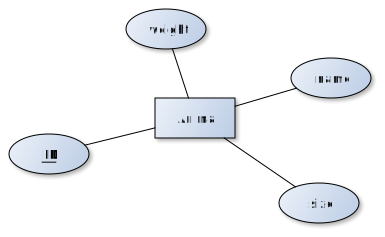
\includegraphics[width=0.9\linewidth]{\currentDir/erd_01}%
\end{center}%
\qENDE{%
Transform the \glsShort{ERD} above to a logical model obeying the relational data model. %
Explain which tables, columns, and constraints you would create.%
}{%
Übertragen Sie das \glsShort{ERD} oben zu einem logischen Modell unter dem relationalen Datenmodell. %
Erklären Sie, welche Tabellen, Spalten und Einschränkungen Sie erstellen würden.%
}%
\end{questionENDE}%
%
\begin{questionENDE}{Modelling}{Modellierung}%
\qENDE{%
Assume that the relationship between tickets and spectators of a concert follows the schema \crowsFoot{ticket}{M1}{spectator}{O1}. %
Every ticket has a date and a price. %
Every spectator has a name. %
Which tables, attributes, and constraints do you need to represent this situation correctly in the relational model?%
}{%
Nehmen Sie an, dass die Beziehung zwischen Eintrittskarten und Besuchern eines Konzerts dem Schema \crowsFoot{Eintrittskarte}{M1}{Besucher}{O1} entspricht. %
Jede Eintrittskarte hat ein Datum und einen Preis.
Jeder Besucher hat einen Namen. %
Welche Tabellen, Attribute und Einschränkungen brauchen Sie, um dieses Situation im relationalen Modell korrekt darzustellen?%
}%
\end{questionENDE}%
%
\begin{questionENDE}{Conceptual to Logical}{Konzeptuell zu Logisch}%
\begin{center}%
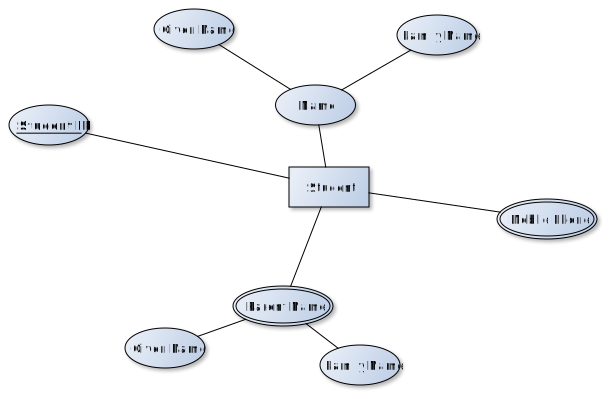
\includegraphics[width=0.9\linewidth]{\currentDir/erd_02}%
\end{center}%
\qENDE{%
Transform the \glsShort{ERD} above to a logical model obeying the relational data model. %
Explain which tables, columns, and constraints you would create.%
}{%
Übertragen Sie das \glsShort{ERD} oben zu einem logischen Modell unter dem relationalen Datenmodell. %
Erklären Sie, welche Tabellen, Spalten und Einschränkungen Sie erstellen würden.%
}%
\end{questionENDE}%
%
\begin{questionENDE}{Modelling}{Modellierung}%
\qENDE{%
Assume that the relationship between salespersons and customers of a furniture store follows the schema \crowsFoot{customer}{OM}{salesperson}{O1}. %
Every customer has a name and address. %
Every salesperson has a worker's number, name, and salary. %
Which tables, attributes, and constraints do you need to represent this situation correctly in the relational model?%
}{%
Nehmen Sie an, dass die Beziehung zwischen Verkäufer und Kunden eines Möbelgeschäftes dem Schema \crowsFoot{Kunde}{OM}{Verkäufer}{O1} entspricht. %
Jede Eintrittskarte hat ein Datum und einen Preis.
Jeder Besucher hat einen Namen. %
Welche Tabellen, Attribute und Einschränkungen brauchen Sie, um dieses Situation im relationalen Modell korrekt darzustellen?%
}%
\end{questionENDE}%
%
%
\begin{questionENDE}{Conceptual to Logical}{Konzeptuell zu Logisch}%
\begin{center}%
\includegraphics[width=0.9\linewidth]{\currentDir/erd_04}%
\end{center}%
\qENDE{%
Transform the \glsShort{ERD} above to a logical model obeying the relational data model. %
Explain which tables, columns, and constraints you would create.%
}{%
Übertragen Sie das \glsShort{ERD} oben zu einem logischen Modell unter dem relationalen Datenmodell. %
Erklären Sie, welche Tabellen, Spalten und Einschränkungen Sie erstellen würden.%
}%
\end{questionENDE}%
%
\begin{questionENDE}{Conceptual to Logical}{Konzeptuell zu Logisch}%
\begin{center}%
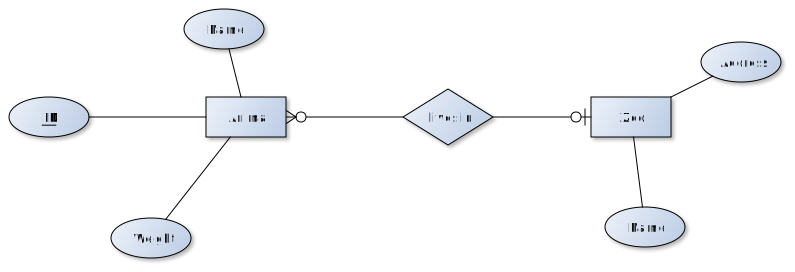
\includegraphics[width=0.9\linewidth]{\currentDir/erd_03}%
\end{center}%
\qENDE{%
Transform the \glsShort{ERD} above to a logical model obeying the relational data model. %
Explain which tables, columns, and constraints you would create.%
}{%
Übertragen Sie das \glsShort{ERD} oben zu einem logischen Modell unter dem relationalen Datenmodell. %
Erklären Sie, welche Tabellen, Spalten und Einschränkungen Sie erstellen würden.%
}%
\end{questionENDE}%
%
\begin{questionENDE}{Conceptual to Logical}{Konzeptuell zu Logisch}%
\begin{center}%
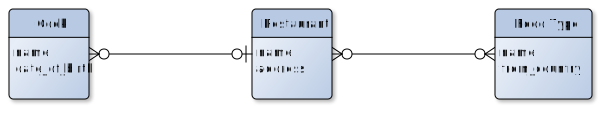
\includegraphics[width=0.9\linewidth]{\currentDir/erd_05}%
\end{center}%
\qENDE{%
Transform the \glsShort{ERD} above to a logical model obeying the relational data model. %
Explain which tables, columns, and constraints you would create.%
}{%
Übertragen Sie das \glsShort{ERD} oben zu einem logischen Modell unter dem relationalen Datenmodell. %
Erklären Sie, welche Tabellen, Spalten und Einschränkungen Sie erstellen würden.%
}%
\end{questionENDE}%
%
\endhsection%
